
\clearpage
\section{La gestion des utilisateurs}

\begin{wrapfigure}[7]{l}{6.5cm}   % [x] Wie manche Zeile soll sich um die Grafik "brechen"
  \vspace{-35pt}      % Grundwert war 20; mit 30 schön oben beim Text ausgerichtet
  \begin{center}
    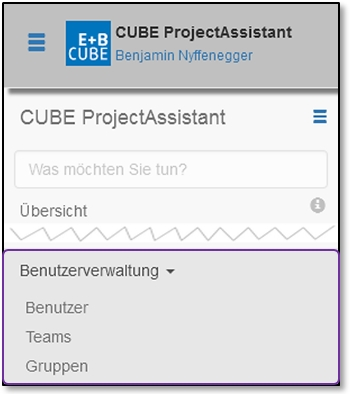
\includegraphics[width=1\linewidth]{../chapters/14_Benutzerverwaltung/pictures/14_Menu_Benutzerverwaltung.jpg}
  \end{center}
  \vspace{-20pt}
  \caption{Utiliser la gestion des utilisateurs}
  \vspace{-10pt}
\end{wrapfigure}

Dans le menu à gauche, sélectionnez l'élément de menu 'Gestion des utilisateurs'. Les sous-éléments 'Utilisateurs', 'Équipes' et 'Groupes' apparaissent.

\vspace{\baselineskip}

La gestion des utilisateurs est uniquement disponible chez les personnes qui ont les droits nécessaires. Elle est utilisée exclusivement par les administrateurs.

\vspace{5cm}  

\textbf{Aperçu :}

\vspace{\baselineskip}

\textbf{Utilisateurs} : Tous les utilisateurs qui ont un point de contact avec CUBE PA sont enregistrés ici. Les attributions aux tags, types de séances, équipes, etc. peuvent se faire ici. De plus, vous pouvez déterminer si un utilisateur doit recevoir un accès à CUBE PA ou s'il doit simplement apparaître dans les champs de sélection (dans les séances, acquisitions, droits d'accès, etc.). Les utilisateurs peuvent être enlevés de la liste des utilisateurs. Un 'élément de contrôle' important est les rôles d’autorisation qui peuvent être attribués à un utilisateur (par exemple administrateur).

\vspace{\baselineskip}

\textbf{Équipes} : Des équipes peuvent être définies ici, et des utilisateurs peuvent y être ajoutés (réglage sous Utilisateurs).

\vspace{\baselineskip}

\textbf{Groupes} : Des groupes peuvent être définis ici. Des utilisateurs, des équipes, et aussi des participants peuvent y être ajoutés. De plus, des droit d'accès spécifiques peuvent être attribués à un groupe (droits de lecture, modification et suppression).

% \clearpage
\subsection{Utilisateurs}
\label{bkm:Ref445362390}

L'aperçu des utilisateurs peut être filtré ou recherché comme les autres aperçus dans CUBE PA. Les utilisateurs listés peuvent être visualisés ou modifiés dans la gestion des utilisateurs \col{(3)}. \textbf{Cependant, il n'est pas possible d'ajouter des utilisateurs ici. Les nouvelles saisies (personnes et unités d'organisation) doivent être effectuées dans la liste d'adresses (voir chapitre \ref{bkm:Ref443738751}.}) \\

\vspace{\baselineskip}

Dans la liste, la date et le temps du dernier login d'un utilisateur sont affichés. 

\begin{figure}[H]
\center{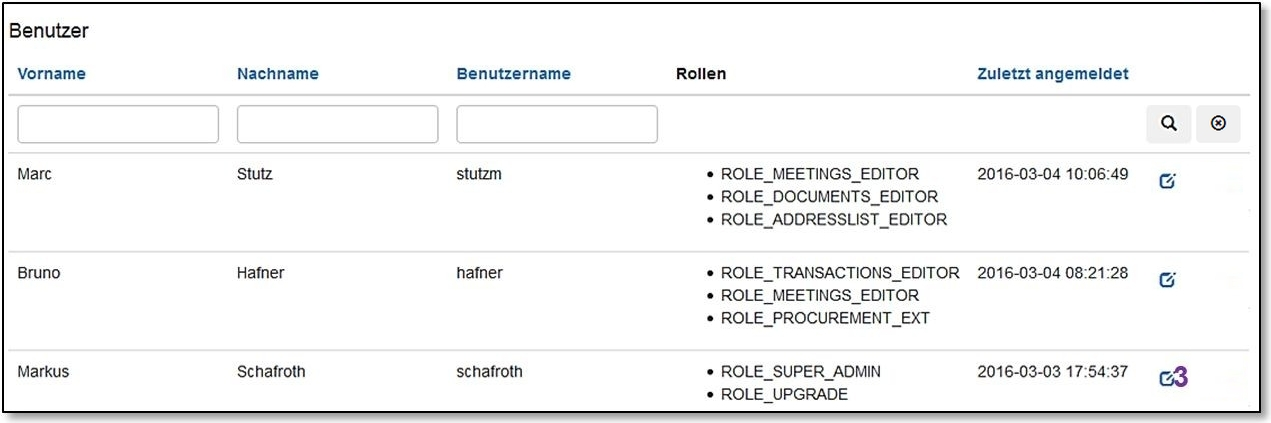
\includegraphics[width=1\linewidth]{../chapters/14_Benutzerverwaltung/pictures/14-1_Benutzeruebersicht.jpg}}
\caption{Aperçu de la gestion des utilisateurs}
% \label{fig:speciation}
\end{figure}

La gestion des utilisateurs et la liste d'adresses réfèrent aux même données dans la base de données. La gestion des utilisateurs, elle, est concentrée sur les utilisateurs qui peuvent se connecter à CUBE PA. Comme expliqué dans le chapitre de la liste d'adresses, saisir une personne dans la liste d'adresses est fait de telle sorte que la personne \textbf{ne puisse pas} se connecter à CUBE PA. La case 'activé' n'est pas disponible. Elle doit être cochée dans la gestion des utilisateurs par une personne autorisée \col{(2)}:

\begin{figure}[H]
\center{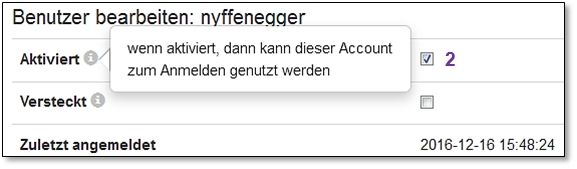
\includegraphics[width=.75\linewidth]{../chapters/14_Benutzerverwaltung/pictures/14-1_BenutzerAktivieren.jpg}}
\caption{Activer un compte d'utilisateur}
% \label{fig:speciation}
\end{figure}

Cliquez sur le symbole d'information 
\includegraphics[height=12pt]{/Icons/Info_Hinweis.jpg}, pour plus d'informations à propos de ces paramètres.

\vspace{-10pt}

% \clearpage
\subsubsection{Rôles}
\label{bkm:Ref445361985}

Les rôles suivants peuvent être attribués à un utilisateur :

\begin{tabular}{|p{7.5cm}|p{7.5cm}|} % {c | p{14cm} l} %{cl}
\hline
\textbf{Rôle} & \textbf{Type} \\
\hline	
ROLE\_IMPORT & ROLE\_USER \\
\hline
ROLE\_IMPORT\_PROJECT\_PLAN\_DATA & ROLE\_IMPORT \\
\hline
ROLE\_IMPORT\_TRANSACTION\_DATA & ROLE\_IMPORT \\
\hline
ROLE\_PROCUREMENT & ROLE\_USER \\
\hline
ROLE\_PROCUREMENT\_EXT & ROLE\_PROCUREMENT \\
\hline
ROLE\_TRANSACTIONS & ROLE\_USER \\
\hline
ROLE\_TRANSACTIONS\_EDITOR & ROLE\_TRANSACTIONS \\
\hline
ROLE\_MEETINGS & ROLE\_USER \\
\hline
ROLE\_MEETINGS\_EDITOR & ROLE\_MEETINGS \\
\hline
ROLE\_HUMANRESOURCES & ROLE\_USER \\
\hline
ROLE\_HUMANRESOURCES\_EDITOR & ROLE\_HUMANRESOURCES \\
\hline
ROLE\_DOCUMENTS & ROLE\_USER \\
\hline
ROLE\_DOCUMENTS\_EDITOR & ROLE\_DOCUMENTS \\
\hline
ROLE\_ADDRESSLIST\_EDITOR & ROLE\_USER \\
\hline
ROLE\_HANDBOOK\_EDITOR & ROLE\_USER \\
\hline
ROLE\_SUPER\_USER & ROLE\_HUMANRESOURCES\_EDITOR, ROLE\_MEETINGS\_EDITOR, \newline ROLE\_TRANSACTIONS\_EDITOR, \newline ROLE\_PROCUREMENT\_EXT, \newline ROLE\_DOCUMENTS\_EDITOR, \newline ROLE\_ADDRESSLIST\_EDITOR, \newline ROLE\_HANDBOOK\_EDITOR \\
\hline
ROLE\_ADMIN & ROLE\_USER, \newline ROLE\_ADDRESSLIST\_EDITOR \\
\hline
ROLE\_SUPER\_ADMIN & ROLE\_ADMIN, \newline ROLE\_IMPORT\_PROJECT\_PLAN\_DATA, ROLE\_IMPORT\_TRANSACTION\_DATA, ROLE\_PROCUREMENT\_EXT,
\newline ROLE\_MEETINGS, \newline ROLE\_MEETINGS\_EDITOR, \newline ROLE\_TRANSACTIONS\_EDITOR, \newline ROLE\_HUMANRESOURCES\_EDITOR,
\newline ROLE\_DOCUMENTS\_EDITOR, \newline ROLE\_ADDRESSLIST\_EDITOR, \newline ROLE\_HANDBOOK\_EDITOR \\
\hline
ROLE\_UPGRADE & ROLE\_USER \\
\hline
\end{tabular}

\begin{itemize}
\item
Le type de rôle~'ROLE\_USER' donne le niveau de droits d'accès le plus bas et est attribué automatiquement à un utilisateur à son premier login.
\item
ROLE\_A: ROLE\_B : Cette attribution de rôles signifie qu'un utilisateur ayant le rôle A a également le rôle B.
\item
ROLE\_X: [ROLE\_Y, ROLE\_Z] : Cette attribution de rôles signifie qu'un utilisateur ayant le rôle X a également les rôles entre crochets (X et Y).
\end{itemize}

Aperçu de la fonction 'Modifier utilisateur' :

\vspace{\baselineskip}
\vspace{\baselineskip}

\begin{wrapfigure}[7]{r}{9cm}
\vspace{-55pt}
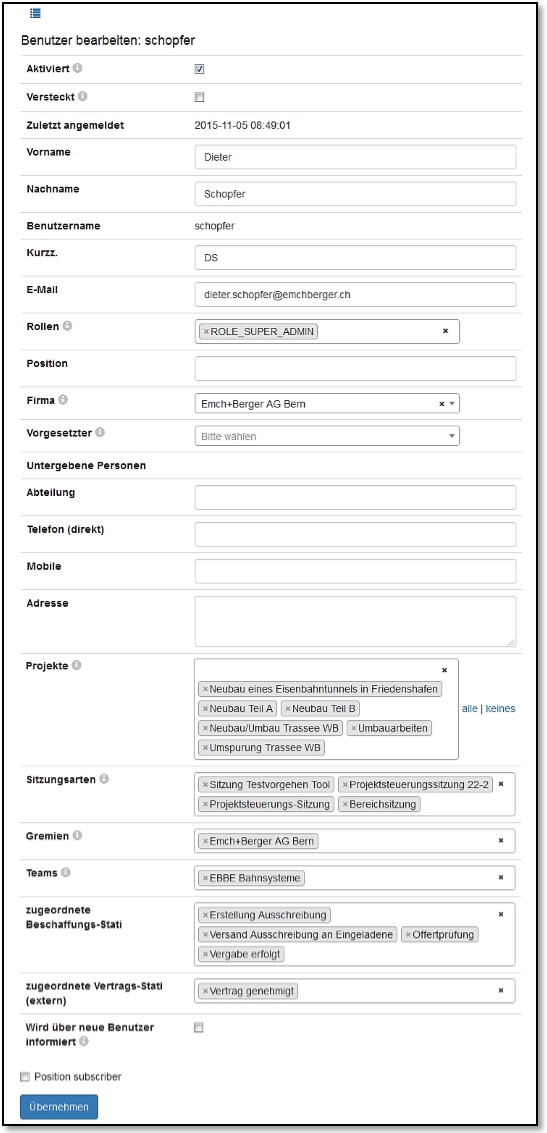
\includegraphics[height=185mm]{../chapters/14_Benutzerverwaltung/pictures/14-1-1_BenutzerBearbeiten.jpg}
% \caption{Status ändern}
\end{wrapfigure}

\begin{small}
\begin{raggedright}

L'utilisateur créé peut se connecter à CUBE PA.

\vspace{\baselineskip}

\mbox{L'utilisateur ne doit pas} 
\mbox{apparaître dans la liste d'adresses}
 et les champs de sélection

\vspace{\baselineskip}

Attribution des différents rôles \
dans CUBE PA (voir chapitre \ref{bkm:Ref445361985})

\vspace{\baselineskip}
\vspace{\baselineskip}
\vspace{\baselineskip}

\mbox{Les utilisateurs peuvent être}
attribués des :

\vspace{\baselineskip}

\begin{itemize}
\item tags
\vspace{\baselineskip}
\vspace{\baselineskip}
\item types de séances
\vspace{\baselineskip}
\item comités
\item équipes
\item processus d'acquisition
\item états dans la \newline fonction d'acquisition
\end{itemize}

\vspace{\baselineskip}


\end{raggedright}
\end{small}

\raggedright{}

\clearpage
\textbf{Indications relatives aux fonctions}

\begin{figure}[H]
\center{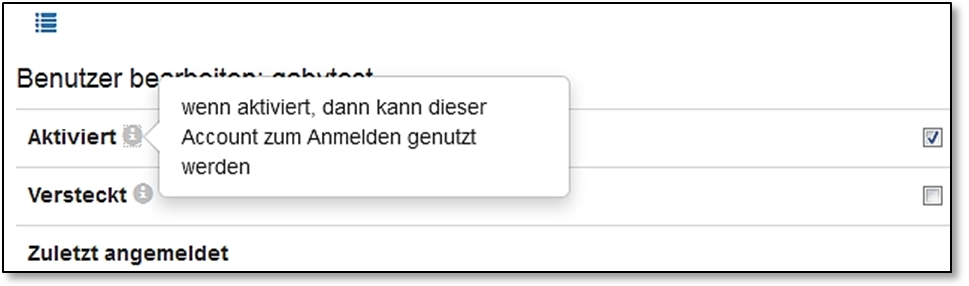
\includegraphics[width=0.6\linewidth]{../chapters/14_Benutzerverwaltung/pictures/14-1-1_Funktionshinweise.jpg}}
\caption{Indications relatives aux fonctions}
% \label{fig:speciation}
\end{figure}

Vous trouverez le symbole 'i' 
\includegraphics[height=12pt]{/Icons/Info_Hinweis.jpg} près de plusieurs champs. Cliquez sur ce symbole pour obtenir une indication relative à la fonction du champ correspondant.

\subsection{Équipes}

Les équipes saisies ici peuvent être attribuées des utilisateurs (voir chapitre \ref{bkm:Ref445362390}).

\begin{figure}[H]
\center{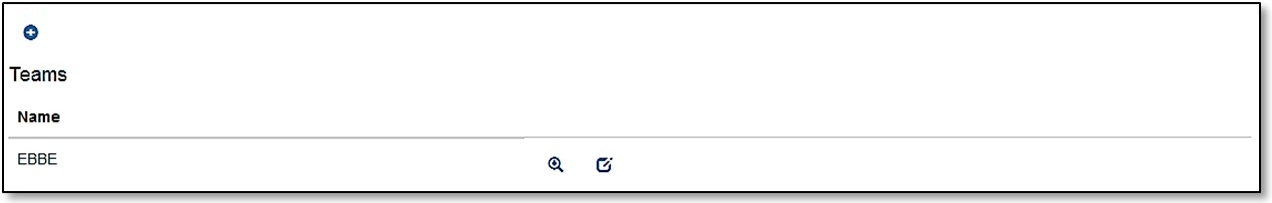
\includegraphics[width=1\linewidth]{../chapters/14_Benutzerverwaltung/pictures/14-2_TeamsUebersicht.jpg}}
\caption{Aperçu des équipes créées}
% \label{fig:speciation}
\end{figure}

\begin{figure}[H]
\center{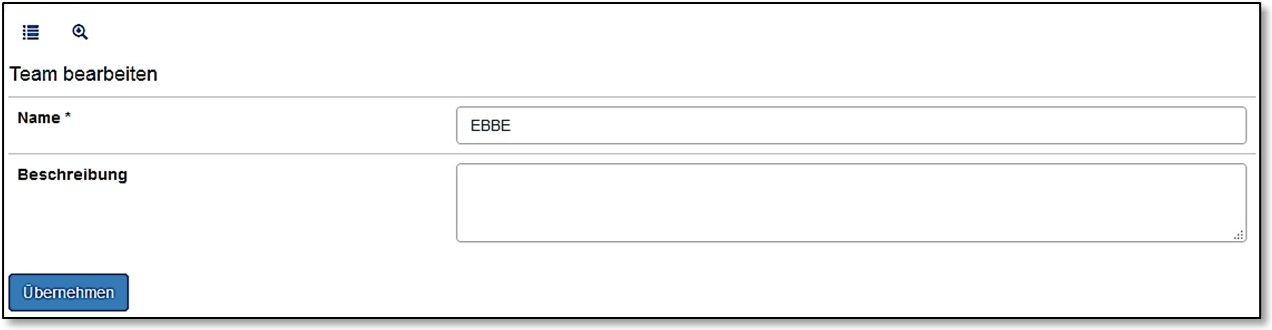
\includegraphics[width=1\linewidth]{../chapters/14_Benutzerverwaltung/pictures/14-2_TeamsBearbeiten.jpg}}
\caption{Mode de modification d'une équipe}
% \label{fig:speciation}
\end{figure}

\clearpage
\subsection{Groupes}

Les groupes peuvent être créés ici. Des utilisateurs, des équipes, et aussi des participants peuvent y être ajoutés. De plus, des droit d'accès spécifiques peuvent être attribués à un groupe (droits de lecture, modification et suppression).

\begin{figure}[H]
\center{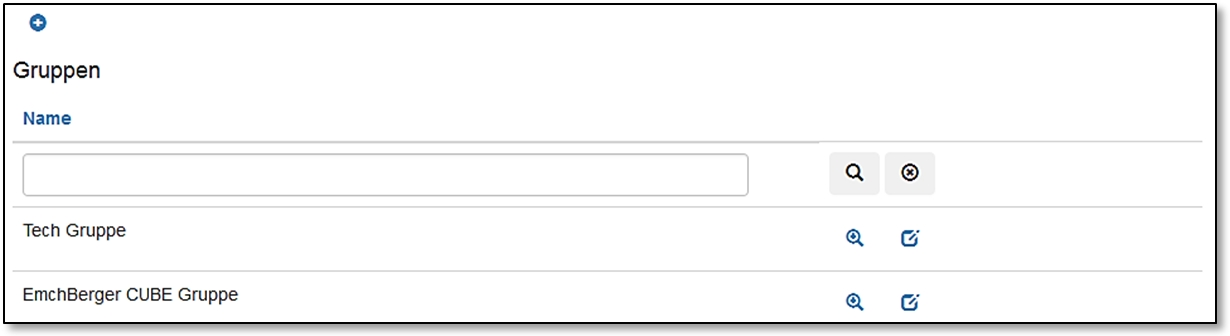
\includegraphics[width=1\linewidth]{../chapters/14_Benutzerverwaltung/pictures/14-3_GruppenUebersicht.jpg}}
\caption{Aperçu des groupes}
% \label{fig:speciation}
\end{figure}

\begin{figure}[H]
\center{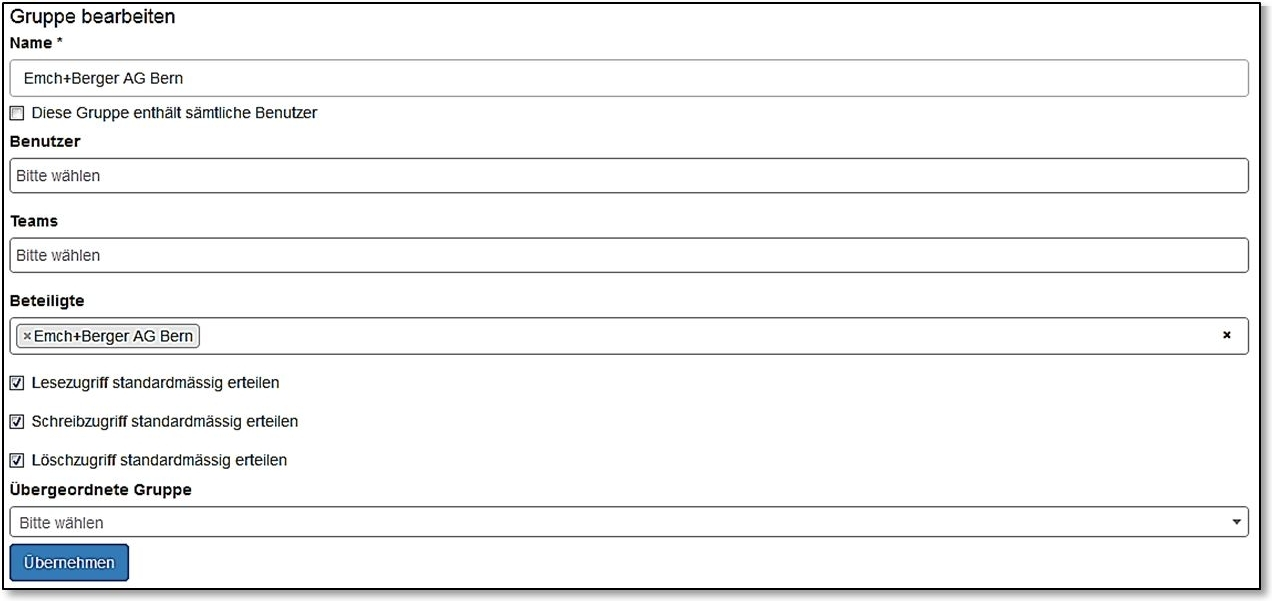
\includegraphics[width=1\linewidth]{../chapters/14_Benutzerverwaltung/pictures/14-3_GruppenBearbeiten.jpg}}
\caption{Mode de modification d'un groupe}
% \label{fig:speciation}
\end{figure}
